\documentclass[12pt]{article}
\usepackage[margin=3cm]{geometry}
\usepackage{graphicx}
\usepackage{float}
\usepackage{url}
\usepackage{listings}
\usepackage{color}

\definecolor{mygreen}{rgb}{0,0.6,0}
\definecolor{mygray}{rgb}{0.5,0.5,0.5}
\definecolor{mymauve}{rgb}{0.58,0,0.82}
\lstset{ %
	xleftmargin=2em,
	backgroundcolor=\color{white},   % choose the background color; you must add \usepackage{color} or \usepackage{xcolor}
	basicstyle=\small,%\footnotesize,        % the size of the fonts that are used for the code
	breakatwhitespace=false,         % sets if automatic breaks should only happen at whitespace
	breaklines=false,                 % sets automatic line breaking
	captionpos=b,                    % sets the caption-position to bottom
	commentstyle=\color{mygreen},    % comment style
	deletekeywords={...},            % if you want to delete keywords from the given language
	escapeinside={\%*}{*)},          % if you want to add LaTeX within your code
	extendedchars=true,              % lets you use non-ASCII characters; for 8-bits encodings only, does not work with UTF-8
	%	frame=single,                    % adds a frame around the code
	keepspaces=true,                 % keeps spaces in text, useful for keeping indentation of code (possibly needs columns=flexible)
	keywordstyle=\color{blue},       % keyword style
	language=C, % the language of the code
	morekeywords={*,...},            % if you want to add more keywords to the set
	numbers=left,                    % where to put the line-numbers; possible values are (none, left, right)
	numbersep=5pt,                   % how far the line-numbers are from the code
	numberstyle=\small\color{mygray}, % the style that is used for the line-numbers
	rulecolor=\color{black},         % if not set, the frame-color may be changed on line-breaks within not-black text (e.g. comments (green here))
	showspaces=false,                % show spaces everywhere adding particular underscores; it overrides 'showstringspaces'
	showstringspaces=false,          % underline spaces within strings only
	showtabs=false,                  % show tabs within strings adding particular underscores
	stepnumber=1,                    % step between two line-numbers. If it's 1, each line will be numbered
	stringstyle=\color{mymauve},     % string literal style
	tabsize=2                  % sets default tabsize to 2 spac                  % show the filename of files included with \lstinputlisting; also try caption instead of title
}

\begin{document}

\begin{titlepage}
	\begin{center}
		
		
		% Upper part of the page. The '~' is needed because \\
		% only works if a paragraph has started.
		\vfill
		
		\textsc{\LARGE Lab 4: Gate Delay and Power}\\[1.5cm]
		
		\Large Adam Sumner\\[0.5cm]
		
		\Large Illinois Institute of Technology\\[0.5cm]
		
		\Large ECE 429-01\\[0.5cm]	
		
		\noindent
		\vfill
		\large \textbf{Lab Date:} October 5\textsuperscript{th}, 2015\hfill
		\large \textbf{Due Date:} October 12\textsuperscript{th}, 2015
		% Bottom of the page
	
		
	\end{center}
\end{titlepage}

\section{Introduction}
The purpose of this lab is to construct a 2-input NAND gate in Virtuoso. Once created, a test circuit will be constructed to simulate and verify the functionality of the gate, and the delay and power measurements will also be analyzed. 
\section{Theory/Pre-Lab}
\subsection{Theory}
Power and delay are a huge concern of VLSI designers when designing a chip. As a consequence, it is important to analyze these characteristics of a design before pushing it into production. Luckily, HSPICE simulation is equipped to measure both, which allows the designer to perform measurements within a SPICE netlist using a \texttt{.measure} statement. For example, to measure the rising and falling delays, this segment of code can be added to the \texttt{*.sp} file: 
\begin{lstlisting}
	.measure tpdr
	+ TRIG v(a) VAL=’0.55’ FALL=1
	+ TARG v(f) VAL=’0.55’ RISE=1
	.measure tpdf
	+ TRIG v(a) VAL=’0.55’ RISE=1
	+ TARG v(f) VAL=’0.55’ FALL=1
\end{lstlisting}

Since a gate is always powered by a supply voltage, power consumption is dependent on the current passing through a gate. Therefore, it is necessary to use a dedicated voltage source to power the gate and since the current will change rapidly when then output is rising/falling, the average power consumption is measured. Using this measure statement:
\begin{lstlisting}
	.measure pwr AVG P(voltage_source) FROM=start_time TO=end_time
\end{lstlisting}
the power consumption of the gate can be measured from start\_time to end\_time.
\subsection{Pre-Lab}
A schematic was to be sketched for a CMOS 2-input NAND gate. It is shown in Figure \ref{fig:pre-lab}.

\begin{figure}
\centering
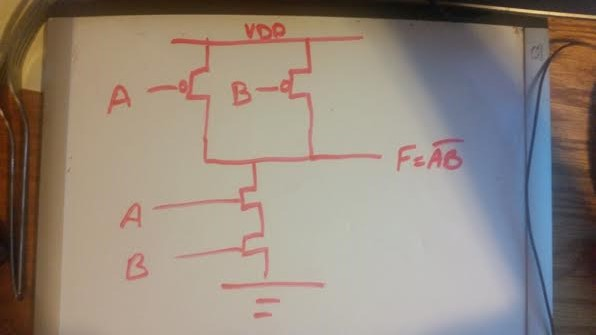
\includegraphics[width=\linewidth]{pre-lab}
\caption{Schematic for 2-Input CMOS NAND Gate}
\label{fig:pre-lab}
\end{figure}

\section{Implementation}
\subsection{Schematics}
\begin{figure}[H]
\centering
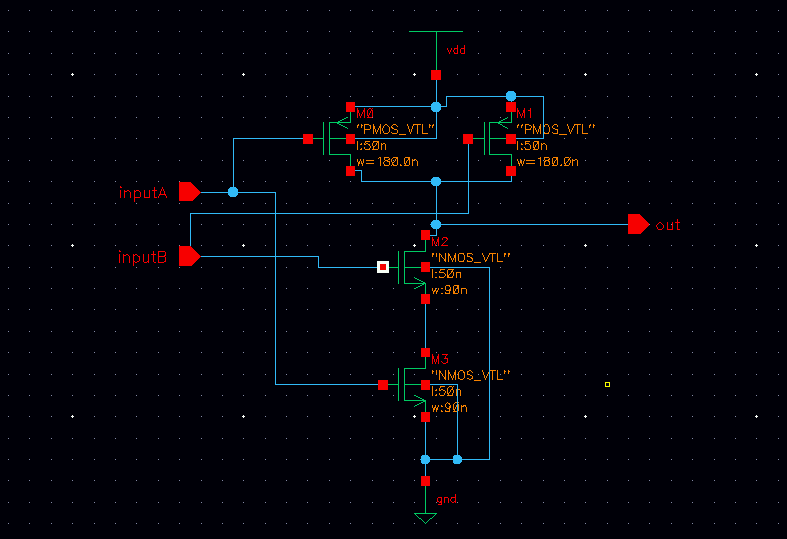
\includegraphics[width=\linewidth]{schematic}
\caption{Schematic for 2-Input CMOS NAND Gate}
\label{fig:schematic}
\end{figure}

\begin{figure}[H]
\centering
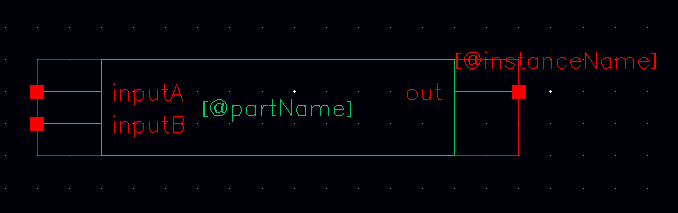
\includegraphics[width=\linewidth]{symbol}
\caption{Symbol for 2-Input CMOS NAND Gate}
\label{fig:symbol}
\end{figure}

\begin{figure}[H]
\centering
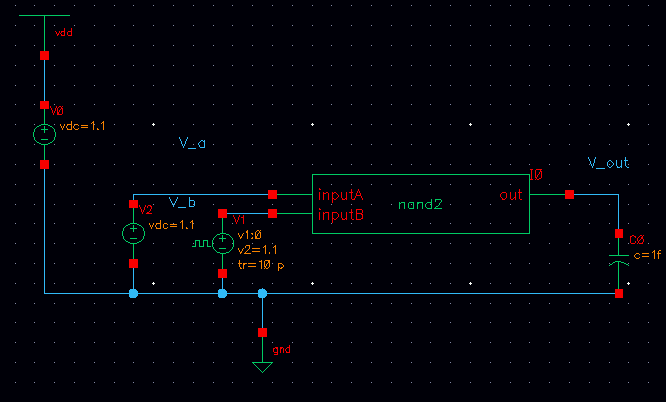
\includegraphics[width=1\linewidth]{test-circuit}
\caption{Test Circuit for Simulation}
\label{fig:test-circuit}
\end{figure}

\subsection{Procedure}
The procedure of this lab involved constructing the 2-Input CMOS NAND gate schematic shown in Figure \ref{fig:pre-lab} in virtuoso. Once created, a symbol was created to easily utilize the newly constructed schematic in other circuits. After this, a test circuit was designed to test the functionality of the NAND gate. This is shown in Figure \ref{fig:test-circuit}. The last step involved simulating the test circuit using HSPICE to verify the functionality of the gate, as well as to measure the delay and power consumption under a load capacitance of 1f, 2f, 4f, and 8f. The results are shown in Tables \ref{tab:1st} - \ref{tab:3rd}.
\subsection{Results}
\begin{table}[H]
	\begin{center}
	\begin{tabular}{ |c|c|c|c|c| }
		\hline
		w=90nm &
		\multicolumn{4}{|c|}{Load Capacitance} \\
		\cline{2-5} l=50nm & 1f & 2f & 4f & 8f \\
		\hline
		Rising Propogation Delay & 5.32e-12 s & 8.56e-12 s & 1.36e-11 s & 2.14e-11 s \\
		\hline
		Falling Propogation Delay & 1.78e-11 s& 2.64e-11 s& 4.24e-11 s& 7.63e-11 s\\
		\hline
		Average Power Consumption & 2.54e-06 W& 3.76e-06 W& 6.21e-06 W& 1.11e-05 W\\
		\hline
	\end{tabular}
	\end{center}
	\caption{Width of 90nm}
	\label{tab:1st}
\end{table}

\begin{table}[H]
	\begin{center}
		\begin{tabular}{ |c|c|c|c|c| }
			\hline
			w=180nm &
			\multicolumn{4}{|c|}{Load Capacitance} \\
			\cline{2-5} l=50nm & 1f & 2f & 4f & 8f \\
			\hline
			Rising Propogation Delay &7.37e-12 s & 1.03e-11 s & 1.47e-11 s & 2.14e-11 s \\
			\hline
			Falling Propogation Delay & 1.06e-11 s& 1.46e-11 s& 2.27e-11 s& 3.85e-11 s \\
			\hline
			Average Power Consumption & 1.66e-06 W& 2.26e-06 W& 3.47e-06 W& 5.73e-06 W \\
			\hline
		\end{tabular}
	\end{center}
	\caption{Width of 180nm}
	\label{tab:2nd}
\end{table}

\begin{table}[H]
	\begin{center}
		\begin{tabular}{ |c|c|c|c|c| }
			\hline
			w=270nm &
			\multicolumn{4}{|c|}{Load Capacitance} \\
			\cline{2-5} l=50nm & 1f & 2f & 4f & 8f \\
			\hline
			Rising Propogation Delay & 1.51e-12 s & 2.93e-12 s & 5.73e-12 s & 9.67e-12 \\
			\hline
			Falling Propogation Delay & 1.01e-11 s& 1.29e-11 s& 1.85e-11 s& 2.90e-11 s \\
			\hline
			Average Power Consumption & 2.29e-06 W& 2.85e-06 W& 4.17e-06 W& 6.58e-06 W\\
			\hline
		\end{tabular}
	\end{center}
	\caption{Width of 270nm}
	\label{tab:3rd}
\end{table}

\begin{figure}[H]
\centering
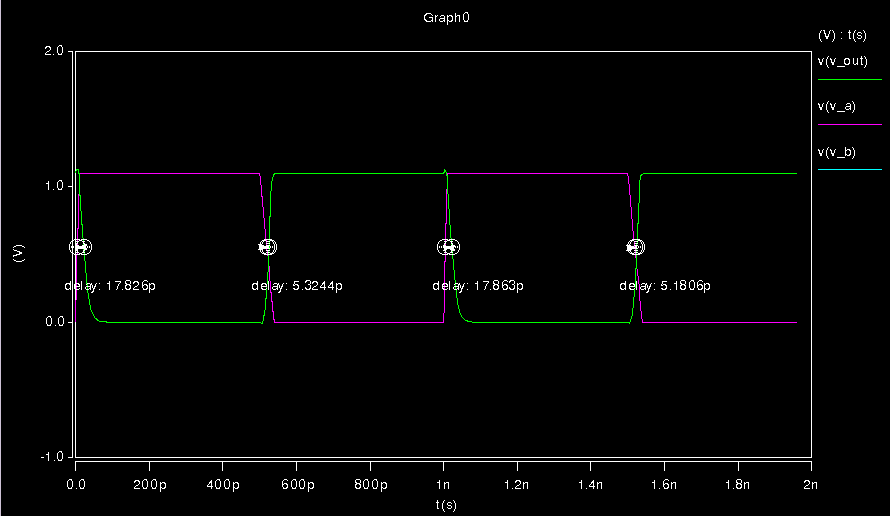
\includegraphics[width=1\linewidth]{00_11_11_00}
\caption{00 $\to$ 11, 11 $\to$ 00 Transition Delay}
\label{fig:00_11_11_00}
\end{figure}

\begin{figure}[H]
\centering
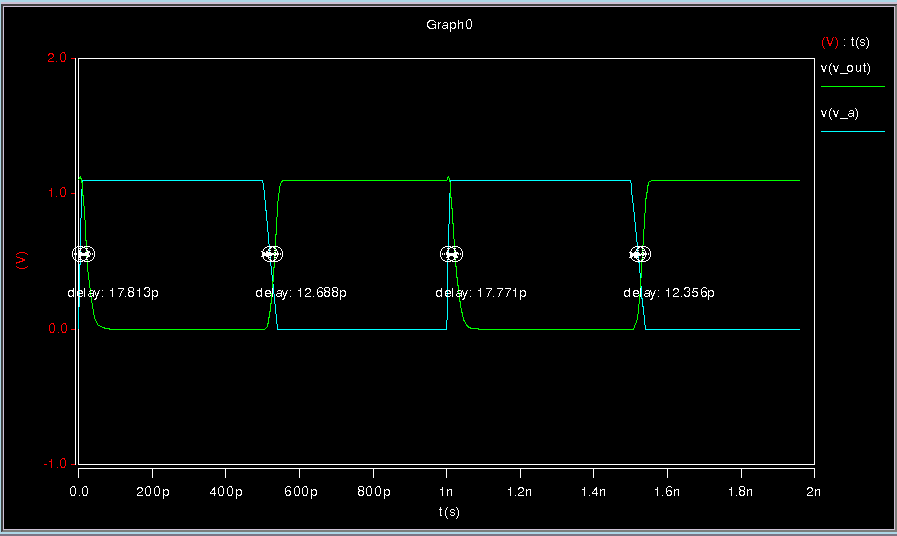
\includegraphics[width=1\linewidth]{01_11_11_01}
\caption{01 $\to$ 11, 11 $\to$ 01 Transition Delay}
\label{fig:01_11_11_01}
\end{figure}

\begin{figure}
\centering
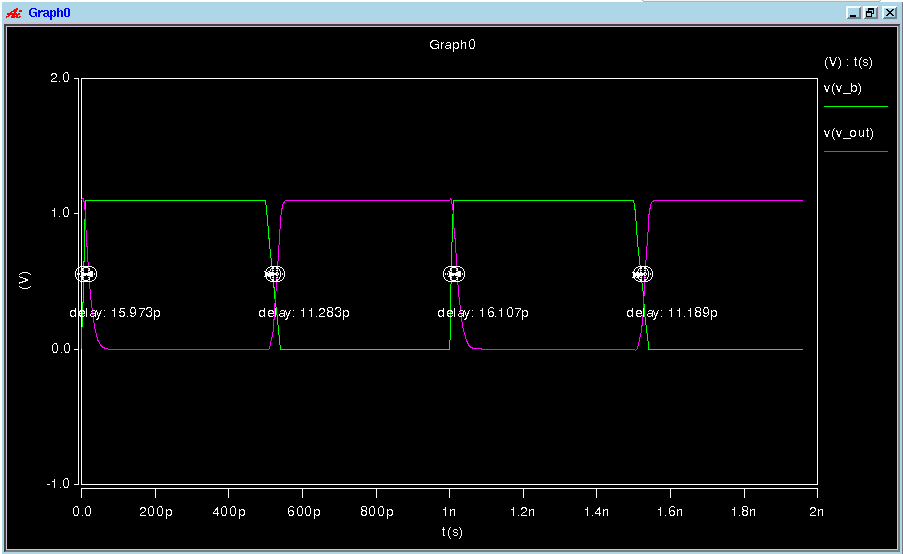
\includegraphics[width=1\linewidth]{10_11_11_10}
\caption{10 $\to$ 11, 11 $\to$ 10 Transition Delay}
\label{fig:10_11_11_10}
\end{figure}

\subsection{Discussion}
The results gathered in this lab demonstrate the correlation between transistor size, load capacitance, and how these attributes affect delay and power consumption. Looking at Table \ref{tab:1st}, as load capacitance was increased the rising delay decreased, the falling delay increased, and the power consumption increased. Table \ref{tab:2nd} shows a similar pattern, while Table \ref{tab:3rd} shows that both delays increased. Nonetheless, in all three cases, power consumption increased linearly as the load capacitance was incremented by factors of 2. Furthermore, it is clear from the data gathered that the functionality of the NAND gate is indeed correct.
\subsection{Questions}
	\begin{enumerate}
		\item \textbf{What input transitions will you expect to have the maximum rising or falling delay? Why? Do the experimental results match your expectations?} I expected 10 $\to$ 11, 11 $\to$ 10 to have the maximum delay. Depending on how the gates are positioned in the NAND gate, I expected when the transition depended on the transistor furthest from the output, there would be a maximum delay. The results showed that 01 $\to$ 11, 11 $\to$ 01 showed a maximum. This is because input A, or the first bit, was furthest from the output.
		
		\item \textbf{Does the relationship between transistor sizes, load capacitances, and propagation delays follow the linear delay model?} Yes. According to the data gathered in this lab, it can be concluded that this relationship follows the linear delay model.
		
		\item \textbf{How does power consumptions change as transistor sizes and load capacitances change?} Power consumption increases
		
		\item \textbf{Among dynamic power, static power, and short circuit power, what are measured in this lab?} Dynamic power is measured in this lab
	\end{enumerate}
%\subsection{Bonus Work}
\section{Conclusions}
Overall the lab was a success. A 2-input CMOS NAND gate was designed and simulated, and its delay and power consumption was measured. It can now be used in further labs and in other circuits that involve 2-input NAND gate functionality.
\end{document}
